%%%%%%%%%%%%%%%%%%%%%%%%%%%%%%%%%%%%%%%%%%%%%%%%%%%%%%%%%%%%%%%%%%%%%%%%%%%%%%%%
% data_set.tex:
%%%%%%%%%%%%%%%%%%%%%%%%%%%%%%%%%%%%%%%%%%%%%%%%%%%%%%%%%%%%%%%%%%%%%%%%%%%%%%%%
\chapter{Analysis Strategy for Long-Lived Particles }
\section{Analysis Strategy}
This analysis searches for delayed isolated photons produced with large transverse momentum. From a theoretical point of view, events containing such a photon will be a clear signal for new physics as such a photon is not expected to be produced from standard model interactions. However, from an experimental point of view, using  timing measurements from  ECAL sub-detector, there are many different sources of isolated, hight \pt photons. A few of these sources which have been identified are high \pt isolated and delayed photons due to timing miss reconstruction and miss-identification, photons produced from cosmic and other beam related effects like beam halo muons bremsstrahlung in the ECAL, and obviously, detector effects like high \pt neutrons by-passing the crystals and hitting directly the photo-detectors like APD and VPT, mimicking the behaviour of isolated, delayed and high \pt photons. The latter kind of photons are called spikes. They are normally isolated, high \pt and their ECAL time measurement show that they arrive early as well as late but with most of them arriving late compared to photons produced at the nominal proton-proton interaction region whose average arrival time at ECAL is 0~ns. These different sources of background makes it a bit challenging to distinguish a possible signal photon from true physics and background photons which are mainly instrumental.
Thus, estimating the background contributions to possible signal sample requires using true proton-proton collision events or data rather than simulated events as is normally done in most physics  analysis. 
Nevertheless, as it is with most hadron collider physics analysis, exploring the use of the number of jets in the event selection can most often reduce dramatically the background contamination to possible signal sample. It is not different with this analysis, as we have employed jet multiplicity both as a physics related quantity for the production of high \pt isolated and delayed photons but also as a detector variable for reducing and at times discriminating  background contribution to possible signal sample.
Our motivation is related to the existence of physics models beyond the SM like the minimal GMSB~(mGMSB) and GGM, where the production of a high \pt isolated, delayed photon in association  with a number of jets constitutes a typical new physics event  which could be produced at the LHC.
Thus using simulated events from mGMSB or GGM model, serves both as a guiding model for the confirmation of a new physics signature at LHC but also as an alternate hypothesis for setting upper limits based on this model in the case that no significant excess over SM prediction is observed.

A typical signal event considered in this analysis for the existence of a neutral massive long-lived particle decaying into a photon is the detection of a late photon arriving at crystals in the ECAL sub-detector of CMS associated with jets with large \MET .  However, the production and decay of this long-lived neutral particle, in our case the neutralino~($\tilde{\chi}^{0}_{1}$), is associated with the production of at least two jets and a weakly interacting gravitino~($\tilde{G}$) as an additional decay product, with a late arrival photon since this is a cascade decay process from a possibly higher mass object into the neutralino and finally to the gravitino. The presence of the gravitino~($\tilde{G}$) is inferred using the transverse momentum imbalance whose magnitude is \MET .
In the  SPS8 minimal GMSB or GGM model with R-parity conservation~(RPC) assumed, SUSY particles are  produced in pairs and so there would be an event having at least a single photon arriving late, associated with at least 2 jets and large \MET . This signal configuration helps in defining and selecting our signal region~(SR) and a control region~(CR) for estimating the contribution to this signal from standard model processes and the detector effects considered as background processes.
\subsection{Signal and Background Modelling}
The SPS8 GMSB and GGM signal event generation begins with the production of Supersymmetry Les Houches Accord~(SLHA) files using the SUSY ISASUSY package written by \cite{Baer}  containing the ISAJET software. The SUSY events are forced to decay according to the SPS8 GMSB and GGM model using the SDECAY decay package. These SLHA files containing information about the SUSY mass spectrum and decay rates is passed through a PYTHIA 6 \cite{pythia6} interface into the CMS software~(CMSSW), in this case CMSSW532patch7, where proton-proton collision at $\sqrt{8}$~TeV events producing SUSY particles events are generated. Their interaction with the CMS detector is simulated using the GEANT4 package \cite{geant4}. Standard Model processes like  multi-jets and $\gamma +$ jets processes produced from strong interactions described by quantum chromodynamics~(QCD) are generated and simulated at leading order cross-sections using PYTHIA 6 and GEANT4 packages respectively.
Digitisation and event reconstruction in terms of its constituent objects like jets, photons, muons and electrons, after its passage and decay in the full CMS detector is later performed still using the CMSSW software.
\subsubsection*{Signal}
The SPS8 mGMSB possible new physics parameter space used for the present physics analysis involves: $\tan\beta = 15$, $sign(\mu) = 1$, and $M_{m} = 2.\cdot \Lambda_{m}$. While $c\tau$ and $\Lambda_{m}$ is used to scan the available parameter space which maximises the sensitivity of the CMS detector to long-lived particles, in this scenario mostly neutralinos~($\tilde{\chi}^{0}_{1}$). The cascade decay of higher mass SUSY particles in the SUSY spectrum to $\tilde{\chi}^{0}_{1}$ allows for signal events with the following constituents:
\begin{itemize}
\item at least one energetic photon,
\item large missing transverse momentum,
\item a number of high transverse momentum jets.
\end{itemize}
\subsubsection*{Background}
QCD multi-jets and $\gamma +$ jet(s) events produced in leading order cross-sections with high \pt range of the photons, serves as background and also for time reconstruction and calibration and for sanity check. Events with $W$  and $Z$ decay  and $t\bar{t}$ with large missing transverse momentum are also generated for serving as sanity check for understanding momentum measurements.
\subsection{Datasets}
The proton-proton collision dataset used in this analysis was collected during 2012 runs at the center of mass energy of  $\sqrt{S} = 8$~TeV  and was collected using the CMS detector totalling and integrated luminosity of 19.1~\fbinv .
\subsubsection*{Data}
The dataset consist is mostly containing events with at least a single photon triggered and only those selected using only luminosity-sections certified as GOOD in the CMS official run file; \textbf{JASON:Cert-8TeVPromptReco-Colllisions12-JASON.txt}. Table \ref{tab:DATA} shows the dataset used in this analysis.

\begin{center}
%\begin{table}[ht]
%\renewcommand\arraystretch{1.2}
\centering
\begin{tabular}{c c}
\hline
Dataset Name & Recorded Luminosity $[\fbinv]$ \\
\hline
 \texttt{/Run2012B/SinglePhoton/EXODisplacedPhoton-PromptSkim-v3 } & 5.1 \\
 \texttt{/Run2012C/SinglePhoton/EXODisplacedPhoton-PromptSkim-v3 } & 6.9 \\
 \texttt{/Run2012D/SinglePhoton/EXODisplacedPhoton-PromptSkim-v3 } & 7.1 \\
\hline
\end{tabular}
\captionof{table}{The dataset name and corresponding integrated luminosity of the data used in the analysis}
\label{tab:DATA}
%\end{table}
\end{center}


\subsubsection*{Background and Signal Monte Carlo}
The Monte carlo ~(MC) samples are produced taking into account the Summer 2012 prescriptions carrying information on the calibration and alignment status of the CMS detector with pile up~(PU) conditions at 8 TeV taking into consideration.
 QCD events are generated with a cross -section ($\sigma$) at leading order~(LO) and normalised to the 19.1 \fbinv integrated luminosity. 50112 events were requested for GMSB signal MC, however, due to an observes reduced lifetime ($c\tau$) observed for these official CMS samples, private sample were generated and simulated covering the same line 8 of the SPS8 mGMSB proposal  while the absence of any MC signal samples for GGM model, meant that we had to privately generate our own samples. The SPS8 mGMSB MC samples are generated to scan $\tilde{\chi}^{0}_{1}$ lifetime $c\tau$ from 250~mm to 12000~mm for each $\Lambda_{m}$ point with $\Lambda_{m}$ ranging from $100$~TeV to $180$~TeV and seen in table \ref{tab:mc_GMSB_sample} while  table \ref{tab:mc_QCD_sample} show the \pt range  for the processed QCD samples.

\begin{center}
%\begin{table}[ht]
%\renewcommand\arraystretch{1.2}
\centering
\begin{tabular}{c c c}
\hline
$c\tau$ (\unit{mm}) & $\sigma_{LO}$ (pb) & number of events\\
\hline
250  & 0.0145 & 50112 \\
500  & 0.0145 & 50112 \\
1000 & 0.0145 & 50112 \\
2000 & 0.0145 & 50112 \\
3000 & 0.0145 & 50112 \\
4000 & 0.0145 & 46944 \\
6000 & 0.0145 & 50112 \\
12000 & 0.0145 & 60000 \\
\hline
\end{tabular}
\captionof{table}{The signal GMSB MC samples used in this analysis}
\label{tab:mc_GMSB_sample}
%\end{table}
\end{center}

\begin{center}
%\begin{table}[ht]
%\renewcommand\arraystretch{1.2}
\centering
\begin{tabular}{c c c}
\hline
$\hat{\pt}$ & $\sigma_{LO}$ (pb) & number of events\\
\hline
 50 $\sim$ 80  & 3322.3  & 1995062 \\
 80 $\sim$ 120 &  558.3  & 1992627 \\
120 $\sim$ 170 &  108.0  & 2000043 \\
170 $\sim$ 300 &   30.1  & 2000069 \\
300 $\sim$ 470 &    2.1  & 2000130 \\
470 $\sim$ 800 &  0.212  & 1975231 \\
\hline
\end{tabular}
\captionof{table}{The $\gamma +$ jets samples used in this analysis}
\label{tab:mc_QCD_sample}
%\end{table}
\end{center}

\section{Event Selection}
The major background events to this analysis are events which are not produced from the nominal proton-proton collisions. These events can be put into four major three major categories; \textit{•} Halo Muons}, \textit{Spikes} and \textit{Cosmic muons}.  In addition to these events, there are also QCD events which mimic the $\tilde{\chi}^{0}_{1} \rightarrow \gamma + \tilde{G}$ decay as a result of photon mis-reconstruction and measurement of fake \MET . Along with QCD events, there are also $\gamma + $ jets events as background where there is the presence of a real isolated photon and a fake \MET is expected due to mis-reconstruction of photons from jets. However, the event topology for $\gamma +$ jets is quite different from that of GMSB events. 
\paragraph*{•}
Another interested possible background contribution, in addition to QCD multi-jets events can come from events with electroweak~(EWK) decay. This include $W \rightarrow e + \nu$ decays, $t\bar{t}$ decays, where the top~(t) decays to a $b$ quark and a $W$ 100\% of the time. The electron is mis-reconstructed as a photon and real \MET is measured due to the presence of the neutrinos~($\nu$).  However, most of these EWK and QCD background contributions have very low jet multiplicity in their events and as a result a selection of events with at least two jets helps to reduce their background contribution to a minimal level prior to additional photon quality selections based on the isolation and electromagnetic shower profile which eventually reduces its contribution to non-existent once photon time acceptance of $t_{\gamma} > 3$~ns is applied.

\paragraph*{}
Cosmic muons, beam halo muons and ECAL spikes can all produced photons large reconstructed time and can contribute largely to \MET measurements since they contribute to \MET calculation which normally measures the \pt of all the detected particles in an event assuming all of these events arise from the nominal proton-proton collision although in practice cosmic muons, beam halo muons, spikes, ECAL and HCAL noise can all contribute to the total sum of the measurable event \pt imbalance but arising from non- nominal collision sources. 
A pre-event selection requiring at least a good vertex, 2 or more jets ECAL spike cleaning, DT time cosmic muon cleaning and CSC tight halo-muon cleaning is shown to be very useful in reducing and estimating the contribution of these important background sources.
\subsubsection{Trigger}
Event selection process begins online using a higher level trigger~(HLT). The HLT trigger used for this analysis during the $\sqrt{S} = 8$~TeV proton-proton collision is the \textit{HLT-DisplacedPhoton65-CaloIdVL-IsoL-PFMET25} seeded by \textit{HLT-L1SingleEG12} level 1 trigger. This trigger was developed primarily for the study of displaced photons. To avoid bias in event selection towards any particular model, this trigger only requires that an accepted event must have an isolated photon with a \pt threshold of 65~GeV/c and a \MET above 25~GeV. In order to study the trigger efficiency and turn-on curve~( where the event selection efficiency becomes very close to 100\%), we avoid  any correlation between the photon and \MET objects selection, by using a single muon dataset~(HLT-IsoMu30) to study the efficiency measurements.
The results of the trigger efficiency measurements are shown in figure \ref{fig:HLTEff} against photon \pt and \MET.

\begin{center}
\centering
%\mbox{
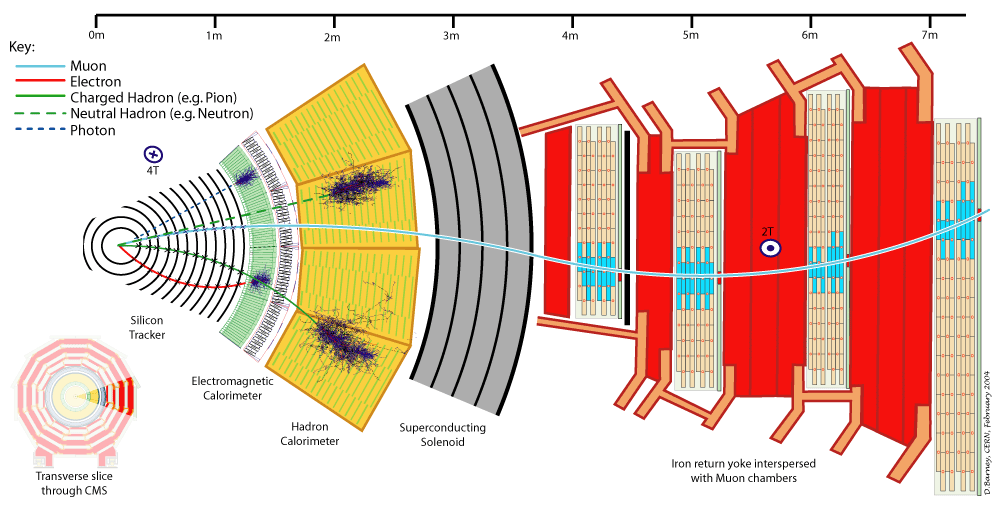
\includegraphics[scale=0.2]{THESISPLOTS/CMS_Slice.png}
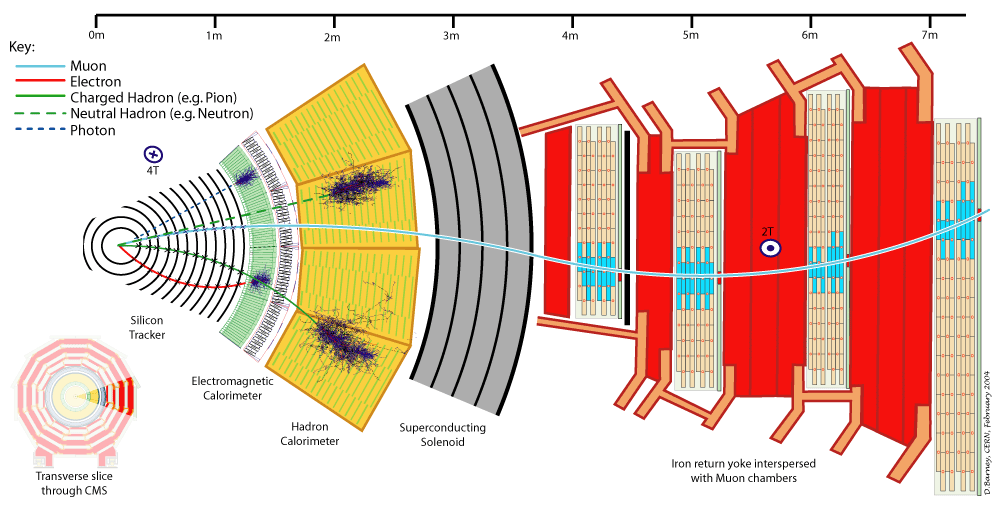
\includegraphics[scale=0.2]{THESISPLOTS/CMS_Slice.png}
\captionof{figure}{Trigger efficiency turn-on curves for photon \pt and $\MET > 25$~GeV~(left) and for \MET with photon $pt > 80$~GeV/c~(right).}
\label{fig:HLTEff}
\end{center}

\subsubsection{Offline Selection}
Offline event selection is directed towards selection of displaced photons with very minimal model dependency in terms of event jet multiplicity as possible. As a result, the event selection requires that the event contains at least one photon. The photon collection in contrast to other analysis, which do not employ the use of ECAL timing as a search variable, is extended to include events categorised as being "out-of-time" during the official super cluster reconstruction. These extension even though allows for the inclusion of possible background from spikes, noise, photons from beam hallo and cosmic muons and detector malfunctions also brings with it photons which are potential signal candidates.
The criteria for photon selections can be found in table \ref{tab:PhotonSel}. 

\begin{center}
%\begin{table}[ht]
\centering
\begin{tabular}{c c }
\multicolumn{2}{c}{\bfseries{Photon identification selection criteria}} \\
  \hline 
  \bfseries{Criteria} & \bfseries{Requirement} \\
   \hline 
 % \texttt{primary vertex number of tracks(vnof)}& $>= 4$ \\
 % \texttt{primary vertex transverse distance to beam}~($d0$) & $ < 2$~cm from CMS center \\
%  \texttt{primary vertex longitudinal distance to beam}~($|z|$) & $ < 24$~cm from CMS center \\
  \texttt{Event leading photon must have} $\pt(\gamma^{1})$  & $ > 80$~ GeV \\
  \texttt{Other photons in event must have} $\pt(\gamma^{>1})$  & $ > 45$~ GeV \\
  
 $|\eta_{\gamma}|$,(\texttt{Barrel Only}),  & $ < 3.0$ ($ < 1.5$) \\
 $S_{minor}$  & $ 0.12 \leq S_{Minor} \leq 0.38$ \\
 \textbf{H/E}  & $ < 0.05$ \\
 
 $\Delta R(\gamma, track)$  & $ > 0.6 $ \\
 
 HCAL Iso  & $ < 4.0 $ \\
 ECAL Iso   & $ < 4.5 $ \\
 Track Iso   & $ < 0.2 $ \\
 Photon Isolation cone size $\Delta R(\gamma, other particle)$ & $< 0.4$ \\
 Topological Spike cuts  & $1 - E_{6}/E_{2} < 0.98$, $ 1 - E_{4}/E_{1} < 0.98$ \\ 
  \hline 
\end{tabular}
\captionof{table}{The photon ID selection as used in this analysis}
\label{tab:PhotonSel}
%\end{table}
\end{center}

The presence of the gravitino~($\tilde{G}$) and jets due to the cascade decay~(Feynman diagram in figure \ref{fig:ProdDecay} of section \ref{Science_Chapter}) of the $\tilde{\chi}^{0}_{1} \rightarrow \gamma + \tilde{G}$ decay process as seen in figure \ref{fig:NeutDecay} requires additional selection of jets and \MET.

\begin{center}
\centering
%\mbox{
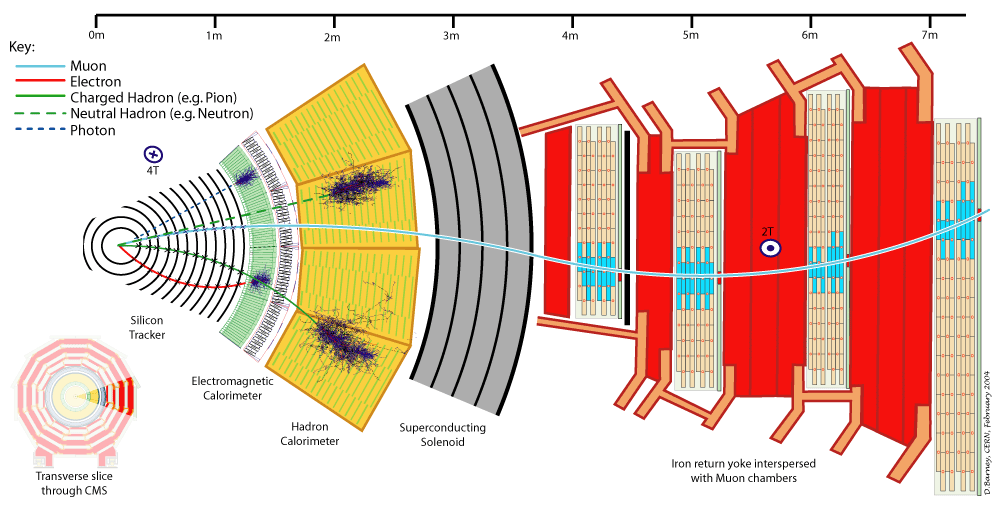
\includegraphics[scale=0.2]{THESISPLOTS/CMS_Slice.png}
\captionof{figure}{Schematic diagram showing $\tilde{\chi}^{0}_{1} \rightarrow \gamma + \tilde{G}$ decay topology within the ECAL volume of the CMS detector.}
\label{fig:NeutDecay}
\end{center}


The jets and \MET selection criteria are based on the particle-flow algorithm. An additional $\MET > 65$~GeV due to the flatness of the HLT trigger efficiency  against \MET ~( see figure \ref{fig:HLTEff}) while  table \ref{tab:JetSel} summarise the jet identification criteria with threshold requirements used for jet selection in this analysis.

\begin{center}
%\begin{table}[ht]
\centering
\begin{tabular}{c c }
\multicolumn{2}{c}{\bfseries{Jet PF identification selection criteria}} \\
  \hline 
  \bfseries{Criteria} & \bfseries{Requirement} \\
   \hline  
\texttt{Jet} \pt & $ > 35$~GeV \\
 \texttt{Number of Jet constituents} & $ > 1$ \\
 \texttt{Charge EM energy fraction~(CEF) } & $ > 0.99$ \\
 \texttt{Neutral Hadron energy fraction~(NHF) } & $ < 0.99$ \\
 \texttt{Neutral EM energy fraction~(NEF) } & $ < 0.99$ \\
 \texttt{If} $|\eta|$ \texttt{of jet is} $ >2.4$, \texttt{Charge Hadron energy fraction~(CHF) } & $ > 0$ \\
 \texttt{If} $|\eta|$ \texttt{of jet is} $ >2.4$, \texttt{Charge multiplicity~(NCH) } & $ > 0$ \\
 $\Delta R(\gamma, jet) = \sqrt{(\phi_{\gamma}-\phi_{jet})^{2} + (\eta_{\gamma}-\eta_{jet})^{2}}$ & $ > 0.3$ \\
\hline
\end{tabular}
\captionof{table}{The Jet ID selection used in this analysis}
\label{tab:JetSel}
%\end{table}
\end{center}


\subsubsection{ECAL Time}
In the current analysis, ECAL time of the photon is the main observable and as a result of pile-up contamination with true photons from nominal proton-proton collisions, a reliable definition for the photon time which is robust to pile up.
The two main definitions for ECAL time studied include:
\begin{itemize}
\item Seed Time: Time from the crystal with higher energy in object super cluster which is not a spike.
\item Cluster Time: Error weighted average time of all the crystals in the seed basic cluster of the object super cluster.
\end{itemize} 

The reconstruction of time as described in chapter 4 is extracted from the pulse shape through a fitting method. The $\chi^{2}$ obtained from the fit determines how well the timing is reconstructed. Thus as a means of rejecting fake photons like jets faking photons as well as spikes, a $\chi^{2} < 4 $ cut is applied to improved on the timing resolution and hence improve on the rejection of anomalous photon.
Figure \ref{fig:spikeVsPhoton} shows a comparison between the pulse shape profile of a spike and that of a normal event from data.

\begin{center}
\centering
%\mbox{
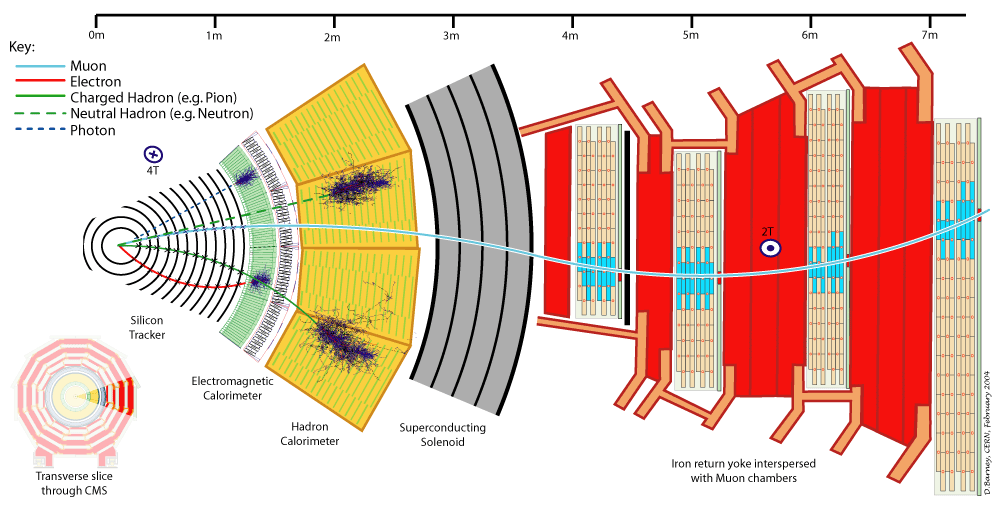
\includegraphics[scale=0.2]{THESISPLOTS/CMS_Slice.png}
\captionof{figure}{Pulse shape profile showing a spike and a real photon time from data.}
\label{fig:spikeVsPhoton}
\end{center}.

In a study performed comparing the timing resolution obtained from cluster time to the seed time, it was observed that also the seed time method is very prone to isolated spikes, its resolution especially for large timing events is much better compared to the cluster time measurement method.
Figure \ref{fig:TIME} shows the timing measurements of photons with $pt > 80$~GeV using either seed time or cluster time. The seed time show a timing resolution of $400$~ps with a narrow time tails compared to $600$ with a broad timing tail obtained from using cluster time.

\begin{center}
\centering
%\mbox{
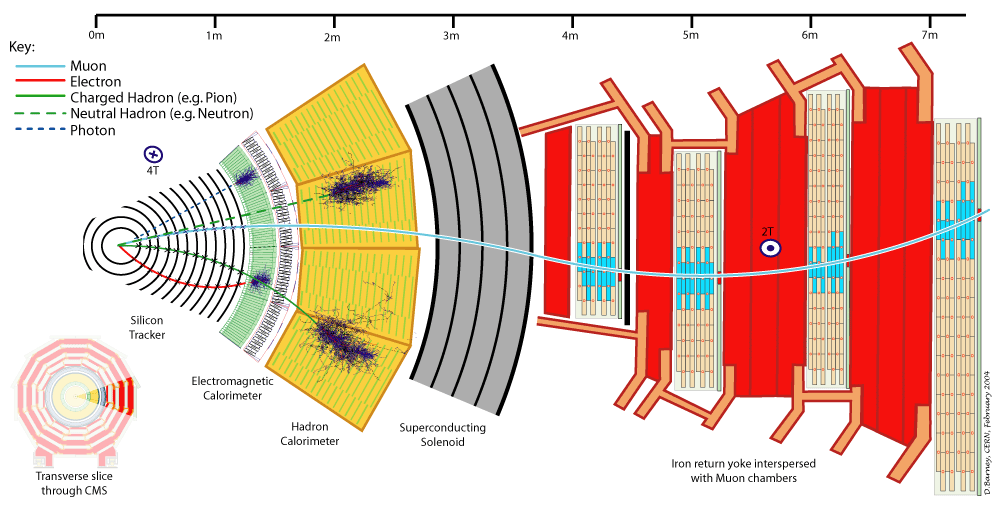
\includegraphics[scale=0.2]{THESISPLOTS/CMS_Slice.png}
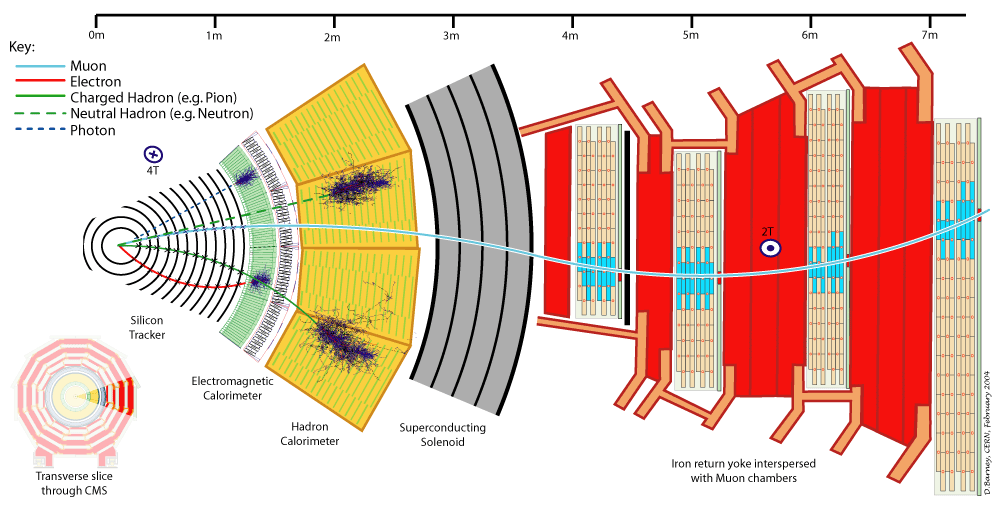
\includegraphics[scale=0.2]{THESISPLOTS/CMS_Slice.png}
\captionof{figure}{Timing distribution of photons with $\pt > 80$~GeV showing timing measurements using seed~(left) and that using cluster time~(right). Resolution from seed time is much better compared to that for cluster time.}
\label{fig:TIME}
\end{center}

Monte Carlo simulation of ECAL timing is very challenging due to the presence of anomalous signals like spikes in data which are not available in MC samples.  Thus in order to study the timing resolution between MC and data, we select events containing only one or two jets and compare this timing distribution to the difference between the Generated time~$(T_{GEN}$) and the MC reconstructed time~($T_{RECO}$) within a timing window of [-2, 2 ]~ns. The difference in peak or mean time between the data and MC $\gamma +$ jet sample is used to smear the reconstructed time of the MC samples to be as comparable to true reconstructed time of data. A difference of about 125~ps is observed between the timing from data and that of MC, and a smearing of of the MC sample shows a close agreement between the smeared reconstructed time of the MC sample to that of data.
Figure \ref{fig:DATAMCTime} shows the this comparison before and after the smearing is applied on the MC samples.

\begin{center}
\centering
%\mbox{
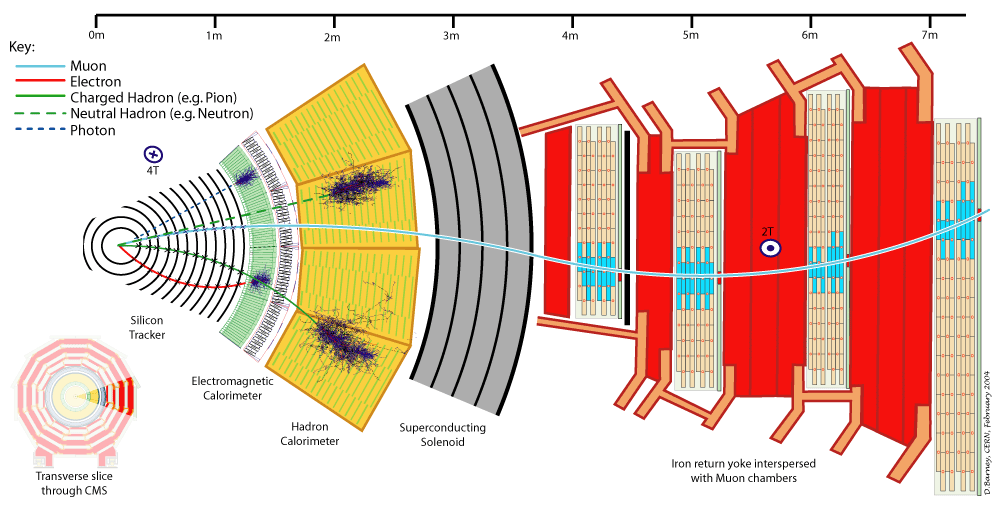
\includegraphics[scale=0.2]{THESISPLOTS/CMS_Slice.png}
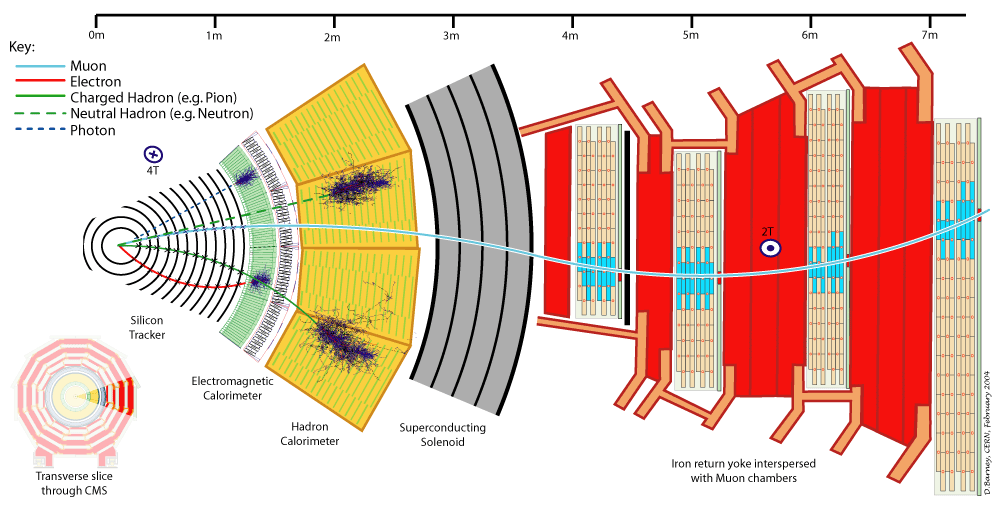
\includegraphics[scale=0.2]{THESISPLOTS/CMS_Slice.png}
\captionof{figure}{Timing distribution of photons with $\pt > 80$~GeV showing timing of data and MC $\gamma +$ jets samples before~(left) and after~(right) smearing of MC is applied.}
\label{fig:TIME}
\end{center}

It is worth noting that the difference of 125~ps between $T^{MC}_{RECO}$ and $T^{DATA}_{RECO}$ compared to 500~ps ECAL timing resolution is not enough to influence event selection, however event distribution in the tails remains a major concern.
\paragraph*{}
The ECAL timing distribution for photons with $pt > 80$~GeV in the ECAL~(barrel and endcap inclusive i.e $|\eta_{\gamma}| < 3.0$) show timing distributions~(see figure \ref{fig:TIMEECAL})

\begin{center}
\centering
%\mbox{
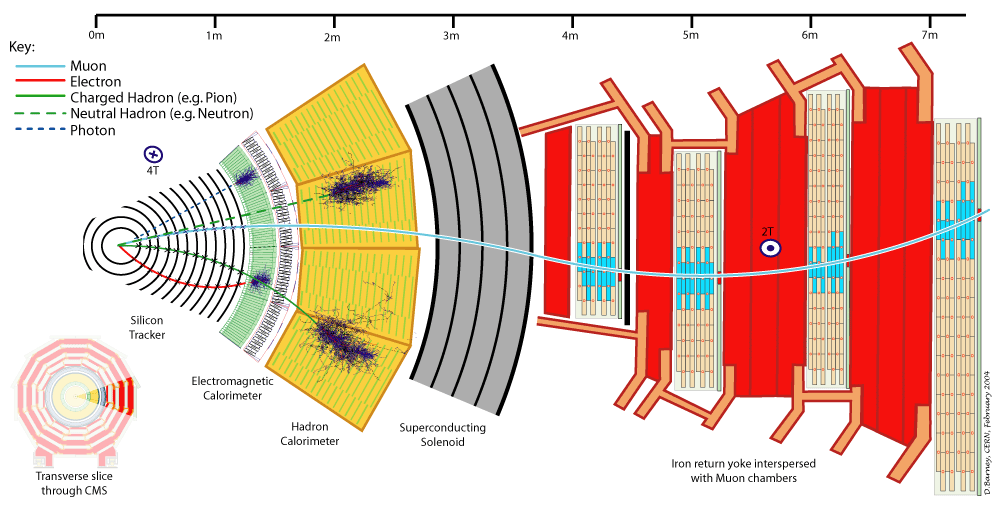
\includegraphics[scale=0.2]{THESISPLOTS/CMS_Slice.png}
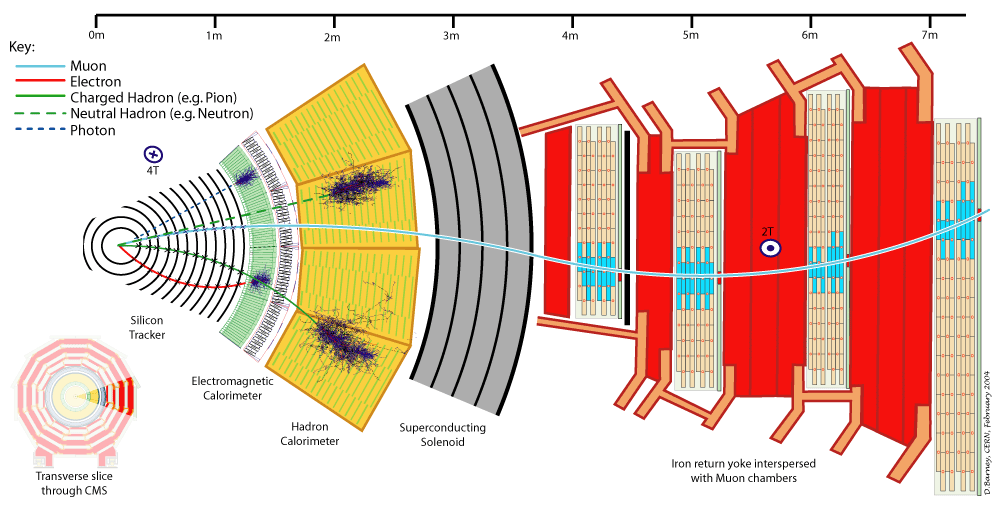
\includegraphics[scale=0.2]{THESISPLOTS/CMS_Slice.png}
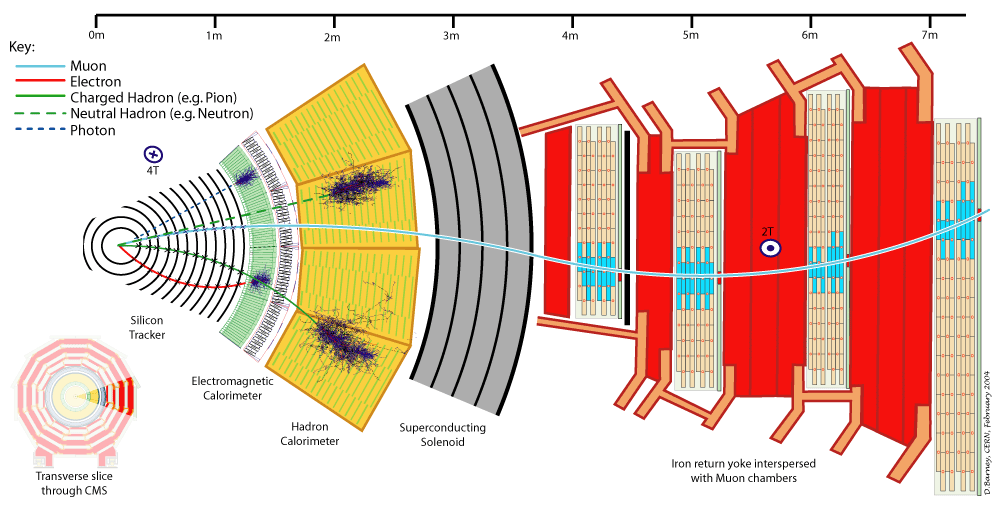
\includegraphics[scale=0.2]{THESISPLOTS/CMS_Slice.png}
\captionof{figure}{ECAL timing distribution of photons with $\pt > 80$~GeV from data showing contributions from main proton-proton collision in EB~(left), EE~(right) and all of ECAL combined~(below). A 2.5~ns timing structure is clearly seen in EE compared to EB}
\label{fig:TIMEECAL}
\end{center}

 with a clear 2.5~ns repeated discrete pattern with most of these photons arriving in the endcap, $ 1.47 < \eta < 3.0$ compared to the barrel, $|\eta| < 1.47$. These are photons originating from collisions of \textit{Ghost} and \textit{Satellite} bunches with either the main proton collision bunch or \textit{Ghost}/\textit{Satellite}. They contribute an irreducible amount to the photon time distribution which is very challenging to reject or estimate quantitatively. A rough estimate can be obtained by looking at ratio of the proton population in the filling profile of the LHC RF cavities as mentioned in section 3.1.5 of chapter 3 which gives a factor $10^{-5}$ compared to contributions from the main proton proton collision. It is observed that their main contribution is towards the endcap crystals as very few photons from these secondary collisions are produced with enough \pt compared to those from main proton bunch collisions. And even if they do, the ratio of photons from these secondary proton collision to that of the main proton-proton collision has an upper bound of  $10^{-5}$. 
Thus, the endcap is not used in this analysis for the reason that these contributions is more in the endcap and the timing resolution in the endcap is relatively poor compared to that of the barrel.
The assumption of the upper bound of $10^{-5}$ is verified and validated using events with $Z\rightarrow e^{+}e^{-}$ as $Z$ events must be produced from main proton-proton collisions rather than  ghost/satellite collisions by studying electron candidates with time within [-2.0, 2.0]~ns window. This will be explain in detail in the background estimation section which follows.


\section{Background Estimation}
A better understanding of the different background contributions to the photon ECAL time is using a two dimensional histogram of the photon $\eta$ and $\phi$ against the photon seed time and the timing distribution for different jet multiplicity events.
This is seen in figure \ref{fig:BKGPLOTS}

\begin{center}
\centering
%\mbox{
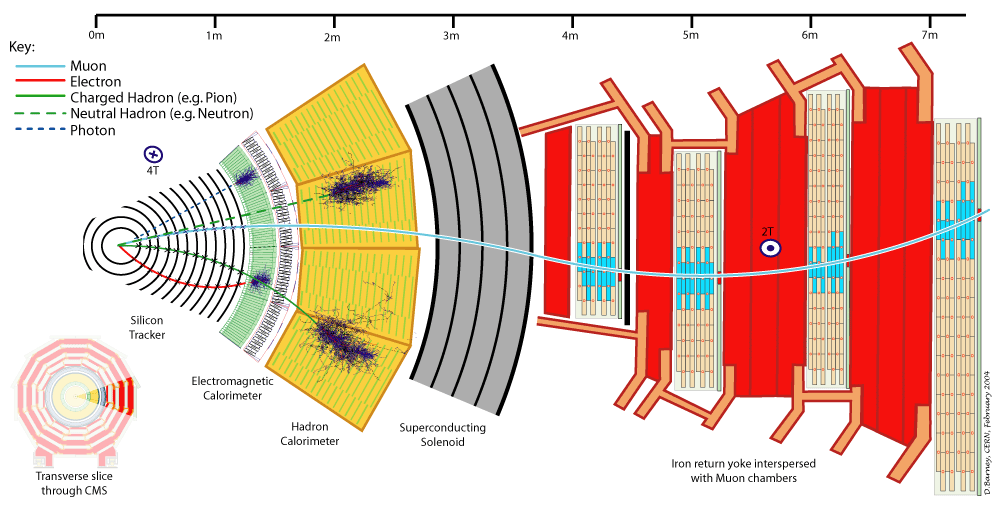
\includegraphics[scale=0.2]{THESISPLOTS/CMS_Slice.png}
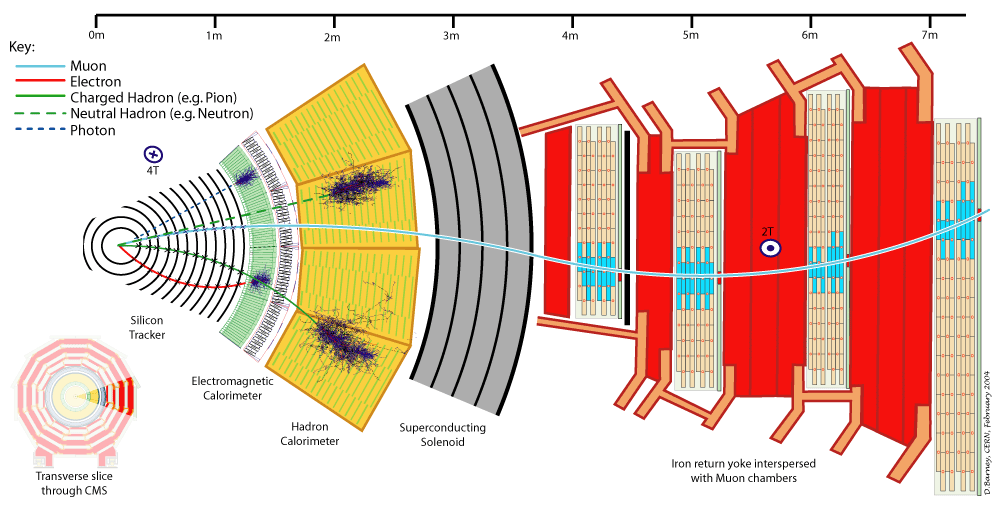
\includegraphics[scale=0.2]{THESISPLOTS/CMS_Slice.png}
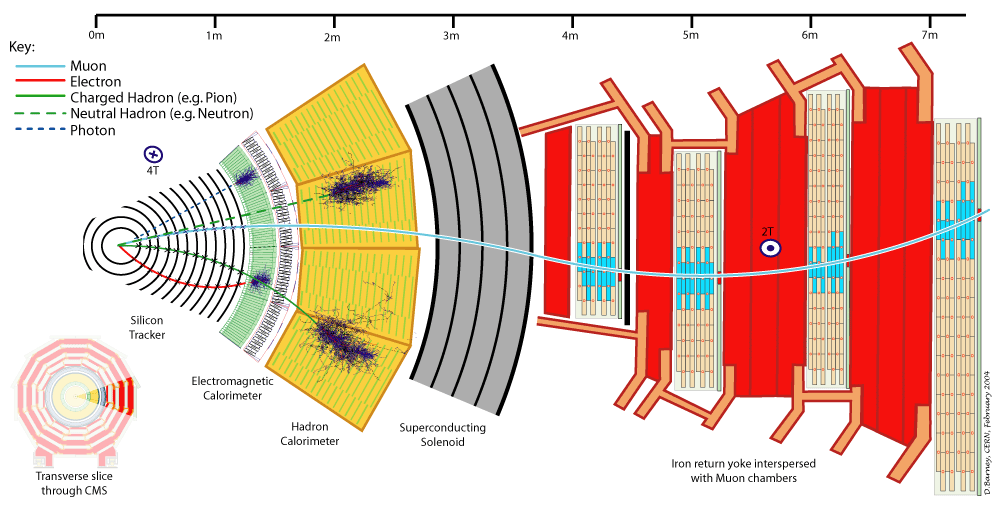
\includegraphics[scale=0.2]{THESISPLOTS/CMS_Slice.png}
\captionof{figure}{ECAL time Vs $\eta$~(left) and ECAL time Vs $\phi$~(right) for photons with $\pt > 80$~GeV from data. The lower plot show the photon timing distribution for events with different jet multiplicity.}
\label{fig:BKGPLOTS}
\end{center}


\subsubsection{Selection Efficiency and Miss-Tag Rate}

\section{Results}

\subsection{Systematics Studies}


\label{Search_Analysis_chapter}